\section{Using STOQS}

\subsection{Operation}

STOQS has been in use at MBARI for over 3 years to help manage and visualize data collected during upper water column measurement campaigns where scientific goals center on improving our understanding of biological processes. The data consist primarily of measurements collected by moving platforms. The platforms have accurate clocks, Global Positioning Sensors and underwater inertial navigation sensors, and one or more instruments that measure parameters such as temperature, salinity, oxygen, nitrate, chlorophyll fluorescence, optical backscatter, and particle sizes. Some platforms can also capture water samples for later laboratory analysis. A typical workflow for is:
\begin{enumerate}
\item Install the STOQS software on a Linux server
\item Vehicles conduct their missions, collecting data
\item Create NetCDF files of the instrument data
\item Construct and execute a STOQS load script
\item Access and visualize data using the STOQS UI
\end{enumerate}


\subsection{Loading Data}

\subsection{Exploring Data}
Collecting high-resolution sections of multidisciplinary data, AUVs offer great potential for understanding marine ecology.  Yet the density and complexity of AUV data challenge efficient and effective exploration.  STOQS is facilitating exploration of AUV data from a variety of experiments.  Here we present an example exploration of AUV data in phytoplankton ecology research.

Occupying the core of the oceanic food web, phytoplankton (microscopic algae) are essential to ocean life, and their photosynthesis supplies about half of humanity’s oxygen needs.  While essential to earth’s biosphere, a small percentage of phytoplankton species can cause harm, for example by producing substances that are toxic to marine life and people.  Studying the ecology of harmful algal blooms (HABs) requires interdisciplinary research over a range of spatial and temporal scales, and AUVs provide excellent observations of phytoplankton patchiness and its relationship to environmental conditions at small to regional scales.  Some AUVs can also acquire whole water samples autonomously targeted on phytoplankton patches, from which subsequent laboratory analyses can reveal phytoplankton identity and toxicity.  Supporting this research, STOQS integrates AUV data on the environment, optical characteristics of the phytoplankton, locations of sampling, and the data derived from shore-side laboratory analyses.

An experiment conducted during fall 2013 in Monterey Bay, California focused on HAB ecology, and it heavily employed AUVs (Fig.~\ref{Fig:JohnsFigureX}).  

\begin{figure}[htbp]
\centering
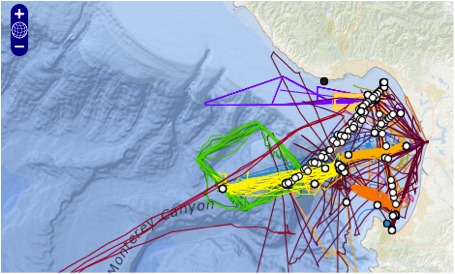
\includegraphics[width=3.3in]{JohnsFigureX.png}
\caption{Map of experiment platform tracks.}
\label{fig:JohnsFigureX}
\end{figure}

One of the primary HAB ecological questions concerns the source of seed populations for bloom events.  Seed populations for blooms may originate within our outside of Monterey Bay.  The first survey by a water-sampling AUV identified spatially separated phytoplankton populations within and outside the bay (Fig.~\ref{Fig:JohnsFigureY}, top panel).  The population outside the bay had much higher chlorophyll fluorescence (left).  The separated phytoplankton populations occupied water of significantly different salinity (Fig.~\ref{Fig:JohnsFigureY}, bottom panel), indicative of different ecological histories.

\begin{figure}[htbp]
\centering
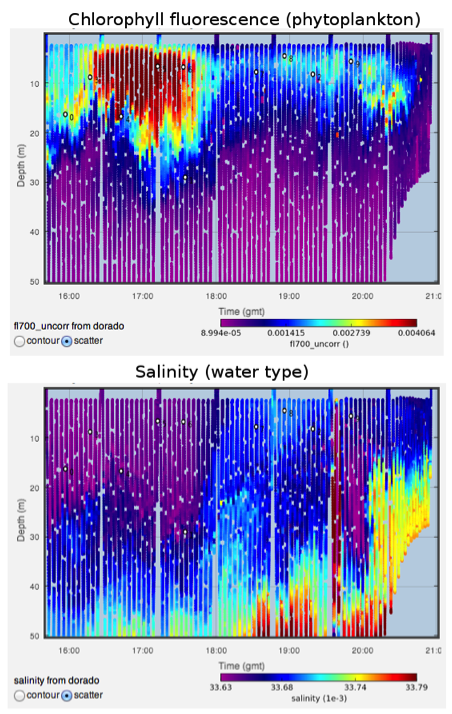
\includegraphics[width=3.3in]{JohnsFigureY.png}
\caption{Vertical sections of chlorophyll fluorescence (top) and salinity (bottom) for an AUV section from offshore (left) to onshore (right) across northern Monterey Bay on 16 September 2013.}
\label{fig:JohnsFigureY}
\end{figure}

Property-property plotting revealed that the spatially separated phytoplankton populations exhibited different optical properties.  The offshore patch exhibited a higher ratio of chlorophyll fluorescence to optical backscattering (Fig.~\ref{Fig:JohnsFigureZ}, high-chlorophyll points identified by the lowest salinity values).

Water samples were acquired by the AUV from both phytoplankton populations (white circles in Fig.~\ref{Fig:JohnsFigureY}).  Examination of these samples by microscopy revealed elevated abundances of a toxigenic species of diatom in the offshore patch.  This simple exploration thus represents the potential for developing optical proxies for phytoplankton ecotypes, as a tool for not only interpretation of data, but also refinement of autonomously targeted sampling by AUVs using optical data in real-time to control sample acquisition.

\begin{figure}[htbp]
\centering
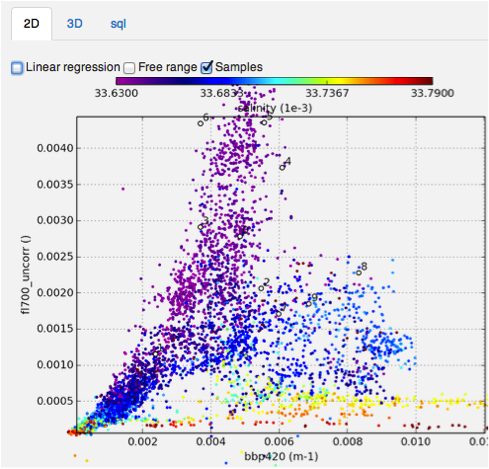
\includegraphics[width=3.3in]{JohnsFigureZ.png}
\caption{STOQS plot of the relationship between optical backscattering (x) and chlorophyll fluorescence (y), colored by salinity, for the AUV section shown inFig.~\ref{Fig:JohnsFigureY}.}
\label{fig:JohnsFigureZ}
\end{figure}

Beyond this simple illustration of AUV data exploration, the fusion of data from many other experiment platforms allows researchers to relate the AUV data to many other observations.

